\chapter{GOTO}

\RU{Оператор GOTO считается анти-паттерном}\EN{GOTO operator considered harmful} 
\cite{Dijkstra:1968:LEG:362929.362947}, 
\RU{но тем не менее, его можно использовать в разумных пределах}
\EN{but nevertheless, can be used resonably} \cite{Knuth:1974:SPG:356635.356640}, \cite[1.3.2]{CBook}.

\RU{Вот простейший пример}\EN{Here is a simplest possible example}:

\lstinputlisting{patterns/065_GOTO/goto.c}

\RU{Вот что мы получаем в}\EN{Here is what we've got is} MSVC 2012:

\lstinputlisting[caption=MSVC 2012]{patterns/065_GOTO/MSVC_goto.asm}

\RU{Так что выражение \IT{goto} просто заменяется инструкцией \JMP, которая работает точно также:
безусловный переход в другое место.}
\EN{So the \IT{goto} statement is just replaced by \JMP instruction, which has the very same
effect: unconditional jump to another place.}

\RU{Вызов второго \printf может исполнится только при помощи человеческого вмешательства,
используя отладчик или модифицирование кода.}
\EN{The second \printf call can be executed only with the help of human intervention, 
using debugger or patching.}\\
\\
\ifdefined\IncludeHiew
\RU{Это также может быть простым упражнением на модификацию кода.}
\EN{This also could be a simple patching exercise.}
\RU{Откроем исполняемый файл в}\EN{Let's open resulting executable in} Hiew: \figref{fig:goto_hiew1}.

\RU{Поместите курсор по адресу где}\EN{Place cursor to the address of} \JMP (\TT{0x410}), 
\RU{нажмите}\EN{press} F3 (\RU{редактирование}\EN{edit}), \RU{нажмите два нуля, так что
опкод будет}\EN{press two zeroes, so the opcode will be} \TT{EB 00}: \figref{fig:goto_hiew2}.

\RU{Второй байт опкода \JMP означает относительное смещение от перехода, 0 означает место
прямо после текущей инструкции.}
\EN{The second byte of \JMP opcode mean relative offset of jump, 0 means the point
right after current instruction.}
\RU{Теперь \JMP не будет пропускать следующий вызов \printf.}
\EN{So now \JMP will not skip second \printf call.}

\RU{Теперь нажмите F9 (запись) и выйдите.}
\EN{Now press F9 (save) and exit.}
\RU{Теперь мы запускаем исполняемый файл и видим это}\EN{Now we run executable and we see 
this}: \figref{fig:goto_result}.

\RU{Подобного же эффекта можно достичь, если заменить инструкцию \JMP на две инструкции \NOP.}
\EN{The same effect can be achieved if to replace \JMP instruction by 2 \NOP instructions.}
\RU{\NOP имеет опкод \TT{0x90} и длину в 1 байт, так что нужно 2 инструкции для замены.}
\EN{\NOP has \TT{0x90} opcode and length of 1 byte, so we need 2 instructions as replacement.}

\begin{figure}[H]
\centering
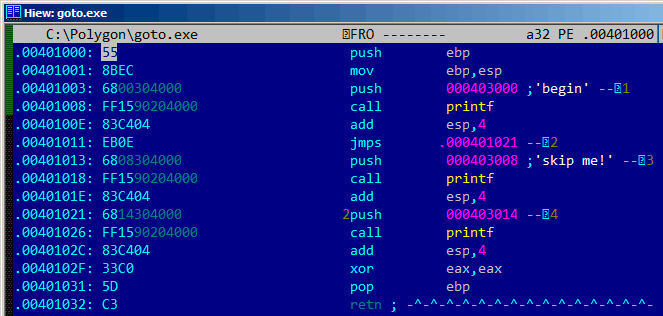
\includegraphics[scale=0.66]{patterns/065_GOTO/hiew1.png}
\caption{Hiew}
\label{fig:goto_hiew1}
\end{figure}

\begin{figure}[H]
\centering
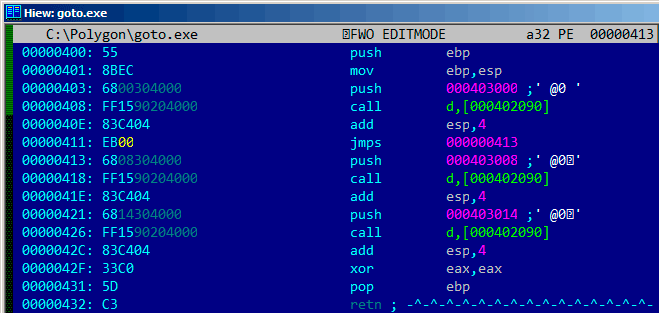
\includegraphics[scale=0.66]{patterns/065_GOTO/hiew2.png}
\caption{Hiew}
\label{fig:goto_hiew2}
\end{figure}

\begin{figure}[H]
\centering
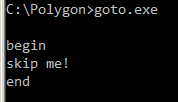
\includegraphics[scale=0.66]{patterns/065_GOTO/result.png}
\caption{\RU{Результат}\EN{Result}}
\label{fig:goto_result}
\end{figure}
\fi

\section{\RU{Мертвый код}\EN{Dead code}}

\RU{Вызов второго \printf также называется ``мертвым кодом'' (``dead code'') 
в терминах компиляторов.}
\EN{The second \printf call is also called ``dead code'' in compiler's term.}
\RU{Это значит что он никогда не будет исполнен}\EN{This mean, the code will never be executed}.
\EN{So when you compile this example with optimization, compiler removing ``dead code'' leaving
no trace of it:}
\RU{Так что если вы компилируете этот пример с оптимизацией, компилятор удаляет ``мертвый
код'' не оставляя следа:}

\lstinputlisting[caption=\Optimizing MSVC 2012]{patterns/065_GOTO/MSVC_goto_Ox.asm}

\RU{Впрочем, строку}\EN{However, compiler forgot to remove the} ``skip me!'' \RU{компилятор 
убрать забыл}\EN{string}.

\ifdefined\IncludeExercises
\section{\Exercise}

\RU{Попробуйте добиться того же самого используя ваш любимый компилятор и отладчик.}
\EN{Try to achieve the same result using your favorite compiler and debugger.}
\fi
